%!TEX TS-program = xelatex

% Шаблон \LaTeX для использования в презентациях
% Автор: Амет Умеров (admin@amet13.name)
% Дата создания: 9 июня 2014 года
% Для удобной работы с файлом рекомендую использовать ОС GNU/Linux, редактор TeXStudio или Atom с плагином language-latex и движок XeLaTeX
% Для построения графиков можно воспользоваться пакетом GeoGebra, а также сайтом http://texample.net/tikz/

\documentclass[xetex,mathserif,serif,t]{beamer} % [t], [c], или [b] --- вертикальное выравнивание на слайдах (верх, центр, низ)
%\documentclass[aspectratio=169,xetex,mathserif,serif,t]{beamer} % Если хотим соотношение сторон 16:9
%%% Преамбула

%%% Темы оформления
% https://www.hartwork.org/beamer-theme-matrix/
% \usetheme{Berkeley}
% \usetheme{Bergen}
% \usetheme{Szeged}

%%% Цветовые схемы
% \usecolortheme{beaver}
% \useinnertheme{circles}
% \useinnertheme{rectangles}
% \usecolortheme{crane}

\usetheme{SevGU} % Тема СевГУ

%%% Работа с русским языком
\usepackage{fontspec}
\usepackage{xunicode}
\usepackage{xltxtra}

\defaultfontfeatures{Ligatures=TeX}
\setmainfont{PT Sans} % http://fonts.ru/public/
%\setmonofont{Courier New}

%%% Beamer по-русски
\newtheorem{rtheorem}{Теорема}
\newtheorem{rproof}{Доказательство}
\newtheorem{rexample}{Пример}

%%% Дополнительная работа с математикой
\usepackage{amsmath,amsfonts,amssymb,amsthm,mathtools} % AMS
\usepackage{icomma} % "Умная" запятая: $0,2$ --- число, $0, 2$ --- перечисление

%%% Номера формул
% \mathtoolsset{showonlyrefs=true} % Показывать номера только у тех формул, на которые есть \eqref{} в тексте.
% \usepackage{leqno} % Нумерация формул слева

%%% Свои команды
\DeclareMathOperator{\sgn}{\mathop{sgn}}

%%% Перенос знаков в формулах (по Львовскому)
\newcommand*{\hm}[1]{#1\nobreak\discretionary{}
{\hbox{$\mathsurround=0pt #1$}}{}}

%%% Работа с картинками
\usepackage{graphicx}    % Для вставки рисунков
\graphicspath{{images/}} % Каталоги с картинками
\setlength\fboxsep{3pt}  % Отступ рамки \fbox{} от рисунка
\setlength\fboxrule{1pt} % Толщина линий рамки \fbox{}
\usepackage{wrapfig}     % Обтекание рисунков текстом

%%% Работа с таблицами
\usepackage{array,tabularx,tabulary,booktabs} % Дополнительная работа с таблицами
\usepackage{longtable}  % Длинные таблицы
\usepackage{multirow}   % Слияние строк в таблице

%%% Другие пакеты
\usepackage{lastpage} % Узнать, сколько всего страниц в документе
\usepackage{soulutf8} % Модификаторы начертания
\usepackage{csquotes} % Еще инструменты для ссылок
% \usepackage[style=authoryear,maxcitenames=2,backend=biber,sorting=nty]{biblatex}
\usepackage{multicol} % Несколько колонок
\usepackage{etoolbox} % Логические операторы

%%% Картинки
\usepackage{tikz}
\usepackage{pgfplots,pgfplotstable}
\usepackage{verbatim,calc,ifthen}


\title{Использование свободного ПО в инфраструктуре облачных услуг}
%\subtitle{Подзаголовок}

%%% Основные параметры презентации
\author[Умеров Амет]{Умеров Амет}
% \author[Иванов И.И.]{Иванов Иван Иванович, СевГУ} % Один автор
\institute[СевГУ]{\vspace{-15ex}Севастопольский государственный университет}
\date{
    %\vspace*{5ex}
    %\includegraphics[width=0.15\textwidth]{images/by-sa.eps}
}

\begin{document}
%%% Содержимое слайдов

\frame[plain]{\titlepage} % Титульный слайд

%-------------------------------------------------------------------------------

\section{Разработка виртуальной инфраструктуры для реализации облачных услуг}

\begin{frame}
\frametitle{\insertsection}
%\framesubtitle{Требования}
Требования:
\begin{itemize}
	\item устранение единых точек отказа %(резервные линки, RAID)
	\item защита от недоброжелателей %(DDoS, флуд)
	\item \textbf{использование свободного ПО по возможности}
	\item документирование
	\item автоматизация
	\item разработка эффективных тарифных планов хостинга
	\item использование в бизнесе
\end{itemize}
\end{frame}

\begin{frame}
\frametitle{\insertsection}
%\framesubtitle{Подпункт 2}
Возможности:
\begin{itemize}
	\item весьма ограниченный бюджет
	\item всего один админ, он же архитектор (некрасиво звучит этот пункт)
	\item отсутствие опыта работы с виртуализацией
	\item желание что-то построить
	\item ??? что-то еще упустил ???
\end{itemize}
\end{frame}

%-------------------------------------------------------------------------------

\section{Общая схема инфраструктуры}

\begin{frame}
\frametitle{\insertsection}
%\framesubtitle{Подпункт 1}
\begin{figure}[h]
	\begin{center}
		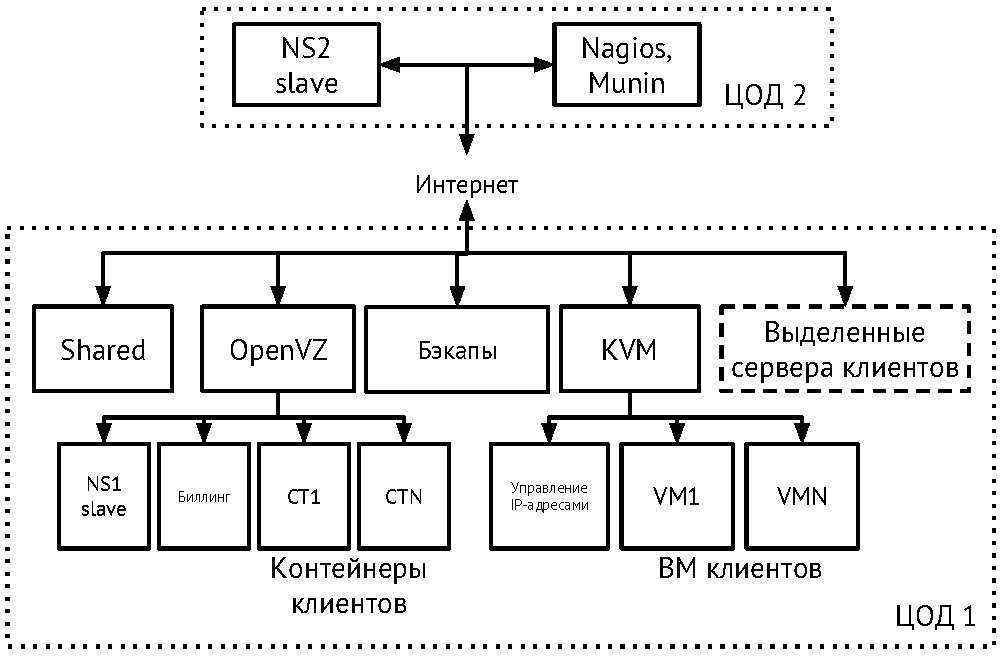
\includegraphics[width=\linewidth]{infrast-scheme}
	 \end{center}
\end{figure}
\end{frame}

%-------------------------------------------------------------------------------

\section{Используемое свободное ПО !(не очень заголовок)}

\begin{frame}
\frametitle{\insertsection}
%\framesubtitle{Подпункт 2}
\begin{itemize}
	\item ОС Linux
	\item мониторинг
	\item виртуализация
	\item автоматизированное управление конфигурациями
	\item скрипты, много скриптов
	\item стандартный стек хостинга
	\item вирусы и malware на хостинге
	\item панели для пользователей виртуальных серверов
\end{itemize}
\end{frame}

%-------------------------------------------------------------------------------

\section{ОС}

\begin{frame}
\frametitle{\insertsection}
\framesubtitle{CentOS 7 (GPL)}
\begin{itemize}
	\item 494 из 500 крупнейших суперкомпьютеров работают на Linux
	\item изобилие серверного ПО
	\item поддержка 6-10 лет (обновление пакетов, исправление уязвимостей и багов)
	\item бесплатно
	\item простая сборка пакетов
	\item драйвера
	\item много документации
\end{itemize}
\end{frame}

%-------------------------------------------------------------------------------

\section{Мониторинг}

\begin{frame}
\frametitle{\insertsection}
\framesubtitle{Nagios → Icinga2 (GPLv2)}
\begin{figure}[h]
	\begin{center}
		\begin{multicols}{2}
		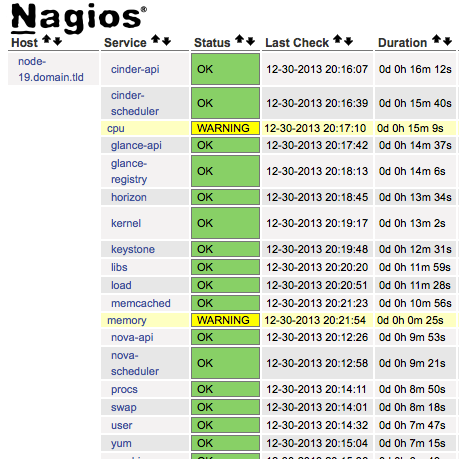
\includegraphics[width=\linewidth]{nagios} \pause \\
		\uncover<2->{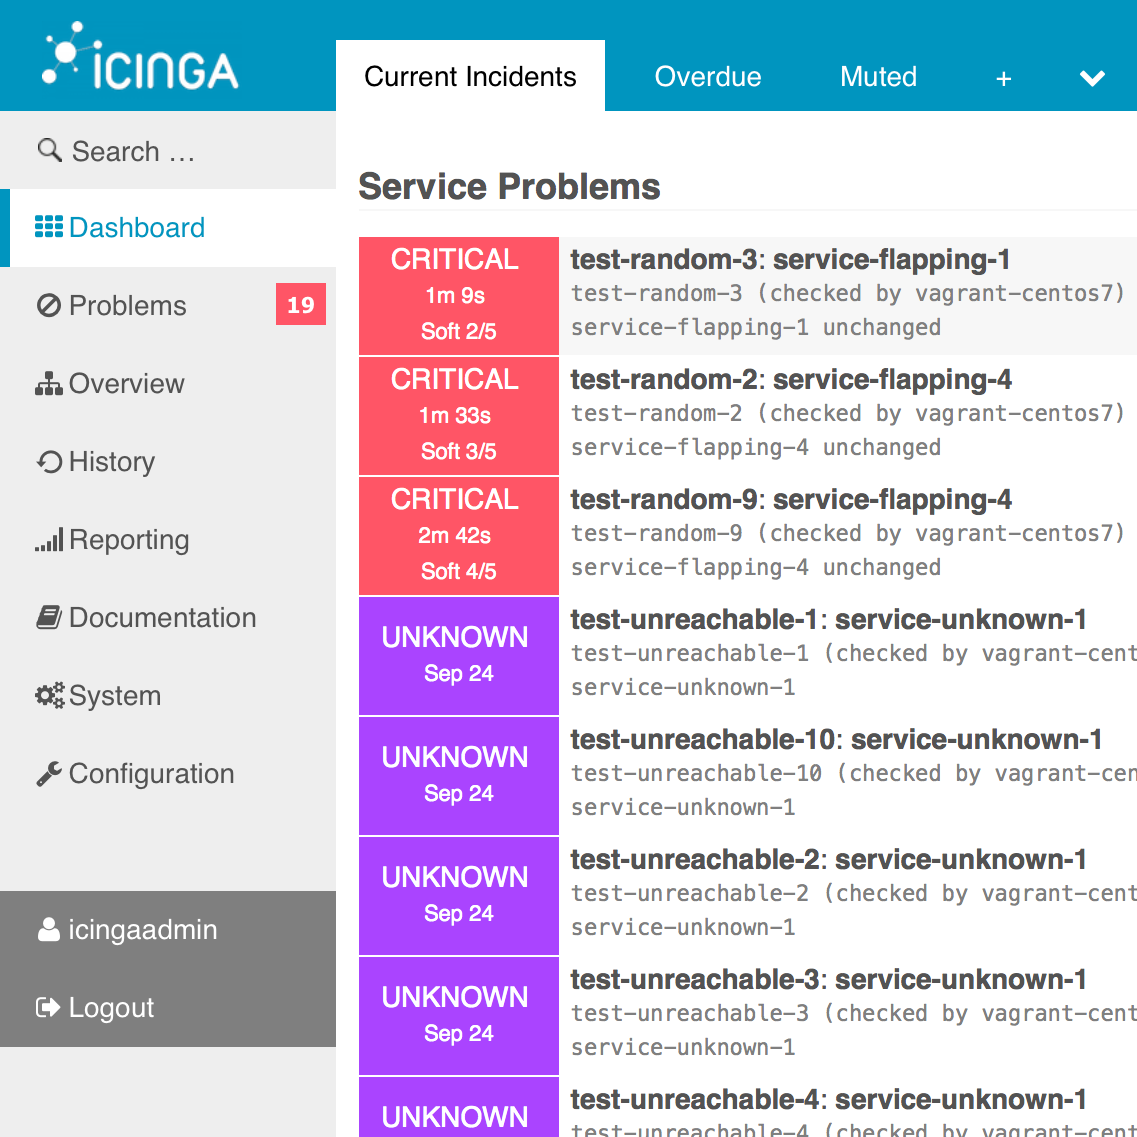
\includegraphics[width=\linewidth]{icinga2}}
		\end{multicols}
	 \end{center}
\end{figure}
\end{frame}

\begin{frame}
\frametitle{\insertsection}
\framesubtitle{Munin (GPL)}
\begin{figure}[h]
	\begin{center}
		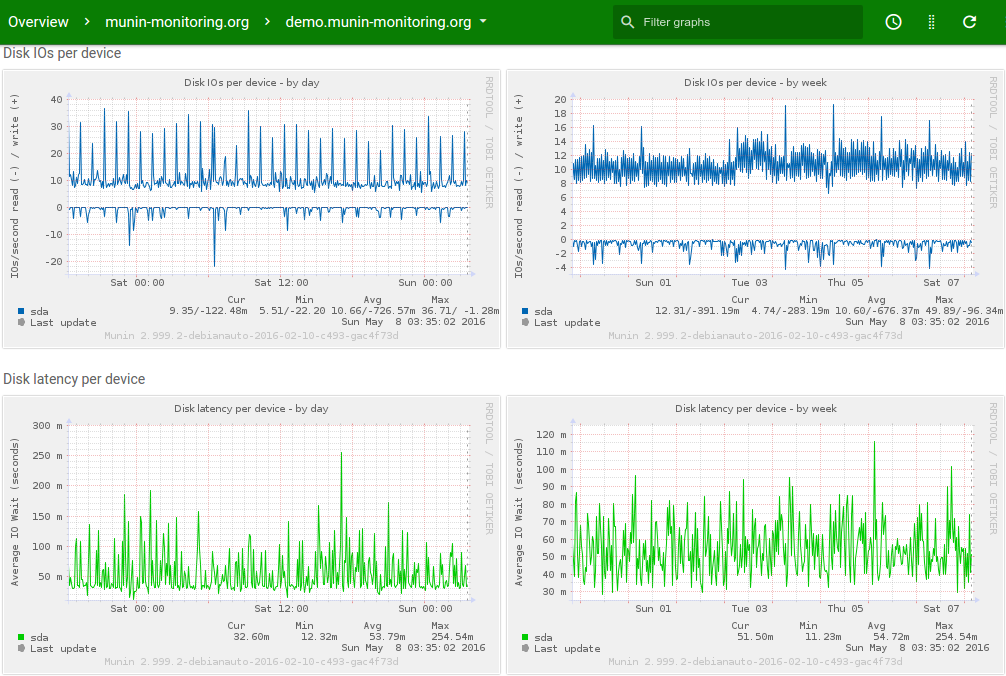
\includegraphics[width=\linewidth]{munin}
	 \end{center}
\end{figure}
\end{frame}

%-------------------------------------------------------------------------------

\section{Управление конфигурациями}

\begin{frame}
\frametitle{\insertsection}
\framesubtitle{Ansible (GPL) + git (GPLv2)}
\begin{figure}[h]
	\begin{center}
		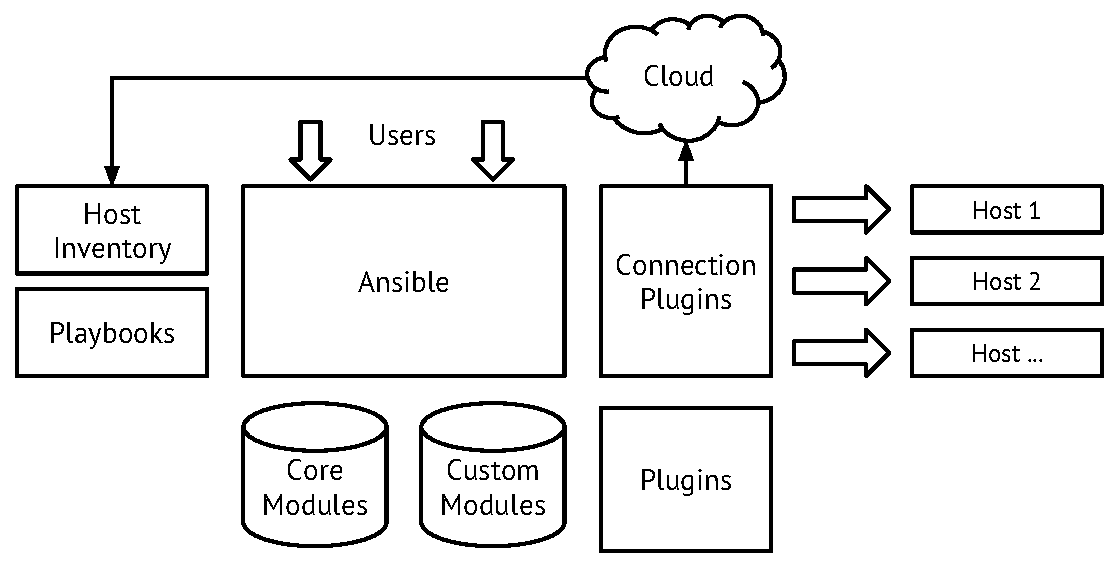
\includegraphics[width=\linewidth]{ansible}
	 \end{center}
\end{figure}
\end{frame}

%-------------------------------------------------------------------------------

\section{Виртуализация}

\begin{frame}
\frametitle{\insertsection}
\framesubtitle{OpenVZ (GPLv2) + KVM (GPL/LGPL)}
\begin{figure}[h]
	\begin{center}
		\begin{multicols}{2}
		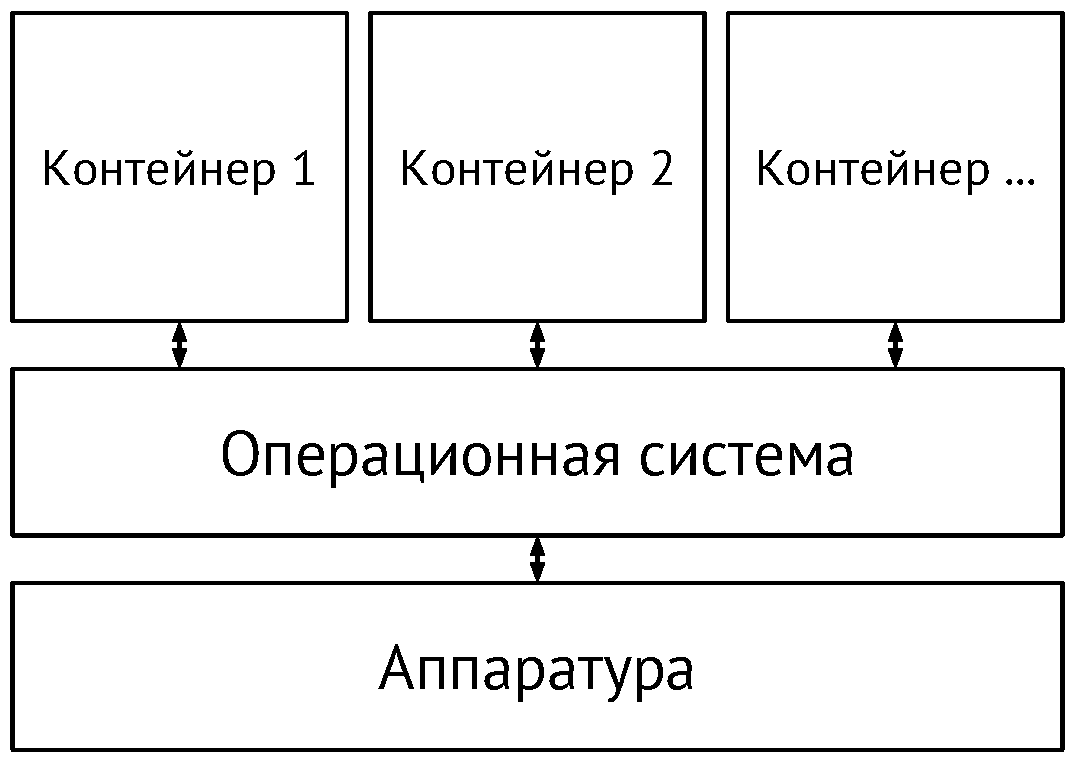
\includegraphics[width=\linewidth]{cont-virt} \\
		OpenVZ \pause \\
		\uncover<2->{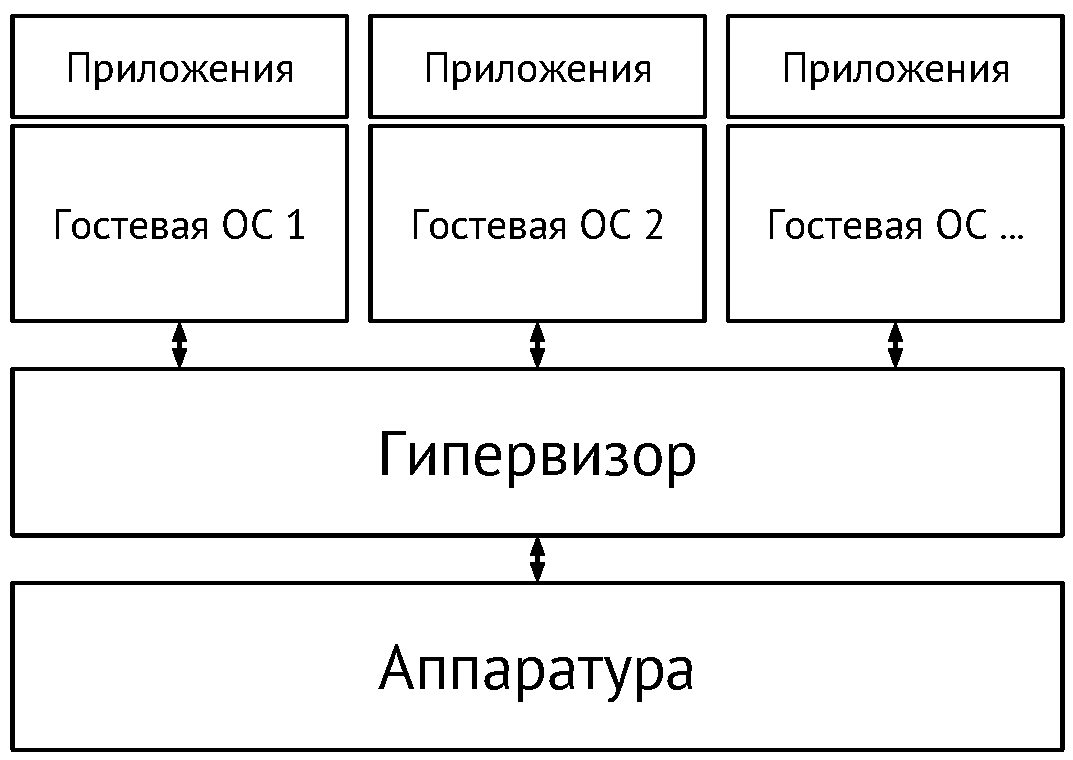
\includegraphics[width=\linewidth]{full-virt}}
		KVM
		\end{multicols}
	 \end{center}
	\end{figure}
\end{frame}

%-------------------------------------------------------------------------------

\section{Стек ПО для хостинга}

\begin{frame}
\frametitle{\insertsection}
%\framesubtitle{LAMP}
\begin{figure}[h]
	\begin{center}
		\begin{multicols}{2}
		
\includegraphics[width=\linewidth]{lamp} \\
		
\includegraphics[width=\linewidth]{mail}
		\end{multicols}
	 \end{center}
	\end{figure}
\end{frame}

%-------------------------------------------------------------------------------

\section{QQQQQQ}

\begin{frame}
\frametitle{\insertsection}
%\framesubtitle{Подпункт 2}
\begin{enumerate}
	\item Элемент 1
	\uncover<2->{\item Элемент 2}
	\uncover<3->{\item Элемент 3*}
\end{enumerate}
\begin{figure}[h]
	\begin{center}
		\begin{multicols}{2}
		
\includegraphics[width=0.3\linewidth]{one} \pause \\
		\uncover<2->{
\includegraphics[width=0.3\linewidth]{two}} \pause \\
		\end{multicols}
		\uncover<3->{
\includegraphics[width=0.15\linewidth]{three}}
	 \end{center}
\end{figure}
\vfill
\footnotesize{* Какая-то сноска}
\end{frame}

%-------------------------------------------------------------------------------

\section{Пункт 3}

\begin{frame}
\frametitle{\insertsection}
\framesubtitle{Подпункт 1}
\begin{itemize}
	\begin{multicols}{2}
	\item Элемент 1
	\item Элемент 1
	\item Элемент 1
	\item Элемент 1
	\item Элемент 1
	\item Элемент 1 \pause \columnbreak
	\item Элемент 2
	\item Элемент 2
	\item Элемент 2
	\end{multicols}
\end{itemize}
\end{frame}

\begin{frame}
\frametitle{\insertsection}
\framesubtitle{Подпункт 2}
\begin{itemize}
	\item Элемент 1
	\begin{itemize}
		\item Подэлемент 1
		\item Подэлемент 2
		\item Подэлемент 3
	\end{itemize}
	\item Элемент 2
	\item Элемент 3
\end{itemize}
\end{frame}

%-------------------------------------------------------------------------------

\section{Выводы}

\begin{frame}
\frametitle{\insertsection}
\begin{itemize}
	\item Элемент 1
	\item Элемент 2
	\item Элемент 3
	\item Элемент 4
\end{itemize}
\end{frame}

%-------------------------------------------------------------------------------

\section{Информационные источники}

\begin{frame}
\frametitle{\insertsection}
\begin{itemize}
	\item Источник 1: \url{http://1.example.com}
	\item Источник 2: \url{http://2.example.com}
	\item Источник 3: \url{http://3.example.com}
	\item Источник 4: \url{http://4.example.com}
\end{itemize}
\end{frame}

%-------------------------------------------------------------------------------

\frame[plain]{\titlepage} % Титульный слайд

\end{document}
